\section{Power Series}

\subsection{Power series and radius of convergence (\S6.1)}

\begin{definition}{Power series and partial sums}{def:power-series}
Fix a centre $x_0\in\mathbb{R}$ and coefficients $(c_n)_{n\ge 0}$. A \emph{power series} (about $x_0$) is
\[
\sum_{n=0}^{\infty} c_n (x-x_0)^n,
\]
with \emph{partial sums} $S_N(x)=\sum_{n=0}^{N} c_n (x-x_0)^n$.
\end{definition}

% --- ADDED: intuition for power series ---
\noindent\textbf{Why ``infinite polynomials''?}
A polynomial $p(x)=a_0+a_1 x+\cdots+a_N x^N$ is the simplest class of function to evaluate, differentiate, and integrate.
A power series generalises this by allowing \emph{infinitely many} terms, giving us the expressive power to represent
transcendental functions ($e^x$, $\sin x$, $\ln(1+x)$, $\dots$) while retaining the easy term-by-term algebra of polynomials.
The price we pay is that we must track \emph{where} the infinite sum converges.

\noindent\textbf{A useful mental model.}
Think of $S_N(x)$ as the ``$N$th polynomial snapshot'' of the full series.
As $N\to\infty$, more and more terms are included; the radius of convergence $R$ tells you the region where these snapshots settle down to a well-defined function.
Outside $|x-x_0|>R$ the snapshots blow up.
% --- END ADDED ---

A power series behaves like a polynomial inside its convergence region, but the region itself must be determined.
The key object is the \emph{radius of convergence} $R\in[0,\infty]$.

\begin{theorem}{Radius of convergence (interval form)}{thm:radius}
For the power series $\sum_{n=0}^{\infty} c_n (x-x_0)^n$, there exists $R\in[0,\infty]$ such that:
\begin{itemize}[leftmargin=*]
\item it converges absolutely for $|x-x_0|<R$;
\item it diverges for $|x-x_0|>R$;
\item when $0<R<\infty$, convergence at the endpoints $x_0\pm R$ must be checked separately.
\end{itemize}
\end{theorem}

% --- ADDED: intuition for the three cases ---
\noindent\textbf{Why exactly three cases?}
At the centre $x_0$ the series trivially converges (every term with $n\ge 1$ vanishes).
Moving away from $x_0$, the terms $|c_n||x-x_0|^n$ grow or shrink depending on the interplay between $|c_n|$ and $|x-x_0|^n$.
If $|c_n|$ decays fast enough (e.g.\ $c_n=1/n!$), the series converges for all $x$ ($R=\infty$).
If $|c_n|$ grows too fast (e.g.\ $c_n=n!$), it diverges for every $x\neq x_0$ ($R=0$).
In between, there is a critical distance $R$ where the behaviour switches from convergence to divergence.
% --- END ADDED ---

\begin{center}
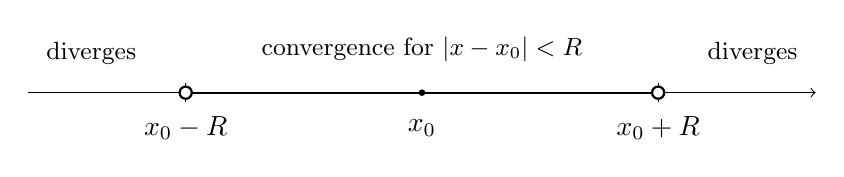
\begin{tikzpicture}
\draw[->] (-5,0) -- (5,0);
\node at (0,-0.45) {$x_0$};
\fill (0,0) circle (1.2pt);
\draw (-3,0.12) -- (-3,-0.12);
\draw (3,0.12) -- (3,-0.12);
\node at (-3,-0.45) {$x_0-R$};
\node at (3,-0.45) {$x_0+R$};
\draw[thick] (-3,0) -- (3,0);
\draw[white, line width=4pt] (-3,0) -- (-3,0); % keep endpoints visually clean
\draw[white, line width=4pt] (3,0) -- (3,0);
\draw[thick, fill=white] (-3,0) circle (2.2pt);
\draw[thick, fill=white] (3,0) circle (2.2pt);
\node at (0,0.55) {\small convergence for $|x-x_0|<R$};
\node at (-4.2,0.5) {\small diverges};
\node at (4.2,0.5) {\small diverges};
\end{tikzpicture}
\end{center}

% --- ADDED: practical computing R ---
\noindent\textbf{Computing $R$ in practice.}
Apply the ratio or root test to $\sum |c_n||x-x_0|^n$ and solve for $|x-x_0|$.
\begin{itemize}[leftmargin=*]
\item \textbf{Ratio test route:} Compute $L=\lim_{n\to\infty}\left|\frac{c_{n+1}}{c_n}\right|$. Then $R=1/L$ (with conventions $1/0=\infty$, $1/\infty=0$).
\item \textbf{Root test route:} Compute $A=\lim_{n\to\infty}\sqrt[n]{|c_n|}$. Then $R=1/A$.
\end{itemize}
Both methods give the same $R$ whenever both limits exist.
% --- END ADDED ---

\begin{examplebox}[title={Worked Example: finding $R$ and the interval (Lecture Ex.~6.3)}]
Find the radius and interval of convergence of $\displaystyle\sum_{n=1}^{\infty}\frac{(-1)^n}{(2n-1)\,2^n}(x-1)^n$.

\smallskip
\textbf{Step 1 (Ratio test).}
Let $a_n=\frac{(-1)^n}{(2n-1)\,2^n}(x-1)^n$. Then
\[
\left|\frac{a_{n+1}}{a_n}\right|
=\frac{2n-1}{2n+1}\cdot\frac{|x-1|}{2}
\xrightarrow[n\to\infty]{}\frac{|x-1|}{2}.
\]
Convergence when $\frac{|x-1|}{2}<1$, i.e.\ $|x-1|<2$, so $R=2$.

Endpoints:
\begin{itemize}[leftmargin=*]
\item At $x=3$: $(x-1)^n=2^n$, so the series becomes $\sum \frac{(-1)^n}{2n-1}$, which converges by the alternating series test.
\item At $x=-1$: $(x-1)^n=(-2)^n$, so the series becomes $\sum \frac{1}{2n-1}$, which diverges.
\end{itemize}
Therefore the interval of convergence is $(-1,\,3]$.
\end{examplebox}

% --- ADDED: extra worked example from lectures (Ex 6.4) ---
\begin{examplebox}[title={Worked Example: endpoint behaviour (Lecture Ex.~6.4)}]
Find $R$ and the interval of convergence for $\displaystyle\sum_{n=0}^{\infty}\frac{(-3)^n x^n}{\sqrt{n+1}}$.

\smallskip
\textbf{Step 1 (Ratio test).}
\[
\left|\frac{a_{n+1}}{a_n}\right|
=3|x|\,\sqrt{\frac{n+1}{n+2}}
\;\xrightarrow[n\to\infty]{}\;3|x|.
\]
Converges when $3|x|<1$, i.e.\ $|x|<\tfrac13$. So $R=\tfrac13$.

\textbf{Step 2 (Endpoints).}
\begin{itemize}[leftmargin=*]
\item $x=-\tfrac13$: series becomes $\sum \frac{1}{\sqrt{n+1}}$, which diverges ($p$-series, $p=\tfrac12<1$).
\item $x=\tfrac13$: series becomes $\sum \frac{(-1)^n}{\sqrt{n+1}}$, which converges (AST: $\frac{1}{\sqrt{n+1}}\downarrow 0$).
\end{itemize}
Interval of convergence: $\bigl(-\tfrac13,\,\tfrac13\bigr]$.
\end{examplebox}
% --- END ADDED ---

% --- ADDED: common mistake on endpoints ---
\begin{commonmistake}[title={Common Mistake: forgetting that endpoints can go either way}]
The ratio/root test is \emph{inconclusive} at $|x-x_0|=R$.
You must substitute each endpoint individually and apply a separate convergence test
(AST, $p$-series, comparison, $n$th-term test, \dots).
The four possible shapes $(\;),\;[\;),\;(\;],\;[\;]$ are all achievable.
\end{commonmistake}
% --- END ADDED ---

\begin{examtip}[title={Exam Focus: a fast workflow for $R$}]
\begin{enumerate}[leftmargin=*]
\item Identify the centre $x_0$ (from $(x-x_0)^n$).
\item Compute $R$ via ratio/root test \emph{ignoring} endpoints.
\item Test endpoints using quick divergence/alternating/comparison logic.
\item State both \textbf{radius} and \textbf{interval} clearly.
\end{enumerate}
\end{examtip}

% --- ADDED: extra exam tip on radius from singularity (Tutorial 12 Method 2) ---
\begin{examtip}[title={Exam Shortcut: radius from nearest singularity (Tutorial~12, Q1 Method~2)}]
For a Taylor series of an analytic function $f$ centred at $a$,
the radius of convergence equals the distance from $a$ to the \emph{nearest singularity}
(real or complex) of $f$.
\begin{itemize}[leftmargin=*]
\item $\ln x$ at $a=2$: singularity at $x=0$, so $R=|2-0|=2$.
\item $e^{2x}$ at $a=3$: entire function, so $R=\infty$.
\item $\sqrt{x}$ at $a=16$: branch point at $x=0$, so $R=|16-0|=16$.
\item $\frac{1}{7x-13}$ at $a=2$: pole at $x=\frac{13}{7}$, so $R=\left|2-\frac{13}{7}\right|=\frac{1}{7}$.
\end{itemize}
This is not a formal exam method (it relies on complex analysis) but is a powerful quick check.
\end{examtip}
% --- END ADDED ---

\subsection{Representing functions by power series (\S6.2)}

A major use-case is to rewrite a function into a form where a known power series applies, then transfer the convergence condition.

% --- ADDED: motivation paragraph ---
\noindent\textbf{The big idea.}
We already know one convergent power series by heart --- the geometric series.
The strategy of this entire section is:
\emph{start from the geometric series, then adapt it using algebra (substitution, multiplication) and calculus (term-by-term differentiation / integration) to represent new functions.}
Every example below follows this pattern.
% --- END ADDED ---

\begin{theorem}{Geometric series}{thm:geometric}
For $|x|<1$,
\[
\frac{1}{1-x}=\sum_{n=0}^{\infty}x^n.
\]
More generally, for constants $A\neq 0$ and $B$,
\[
\frac{1}{A-B(x-x_0)}=\frac{1}{A}\cdot \frac{1}{1-\frac{B}{A}(x-x_0)}
=\frac{1}{A}\sum_{n=0}^{\infty}\left(\frac{B}{A}\right)^n (x-x_0)^n,
\]
valid when $\left|\frac{B}{A}(x-x_0)\right|<1$.
\end{theorem}

% --- ADDED: step-by-step rewriting recipe ---
\noindent\textbf{Rewriting recipe (step by step).}
Given a rational function $\frac{C}{\alpha + \beta x}$:
\begin{enumerate}[leftmargin=*]
\item Factor out the constant from the denominator so you have $\frac{C}{\alpha}\cdot\frac{1}{1+\frac{\beta}{\alpha}x}$.
\item Recognise $\frac{1}{1+\frac{\beta}{\alpha}x}=\frac{1}{1-\bigl(-\frac{\beta}{\alpha}x\bigr)}$.
\item Apply the geometric series with $u=-\frac{\beta}{\alpha}x$.
\item The convergence condition is $|u|<1$, i.e.\ $|x|<\frac{|\alpha|}{|\beta|}$.
\end{enumerate}
% --- END ADDED ---

\begin{keyformula}[title={Key Formula: ``rewrite to geometric form'' pattern}]
Aim to express $f(x)$ as
\[
f(x)=\frac{C}{1-u(x)},
\quad\text{so that}\quad
f(x)=C\sum_{n=0}^{\infty}u(x)^n
\quad\text{when }|u(x)|<1.
\]
Then \textbf{the inequality $|u(x)|<1$ becomes your interval condition}.
\end{keyformula}

\begin{examplebox}[title={Worked Example: rational function to power series}]
Find a power series for $\displaystyle f(x)=\frac{3}{2+x}$ about $x_0=0$ and its interval of convergence.

Rewrite:
\[
\frac{3}{2+x}=\frac{3}{2}\cdot \frac{1}{1+\frac{x}{2}}
=\frac{3}{2}\cdot \frac{1}{1-\left(-\frac{x}{2}\right)}.
\]
Using Theorem~\ref{thm:geometric},
\[
\frac{3}{2+x}=\frac{3}{2}\sum_{n=0}^{\infty}\left(-\frac{x}{2}\right)^n
=\sum_{n=0}^{\infty} \frac{3(-1)^n}{2^{n+1}}x^n,
\]
valid when $\left|-\frac{x}{2}\right|<1$, i.e.\ $|x|<2$. Thus the radius is $R=2$.
\end{examplebox}

% --- ADDED: extra worked example with non-zero centre (Lecture Ex 6.7) ---
\begin{examplebox}[title={Worked Example: expansion about a non-zero centre (Lecture Ex.~6.7)}]
Find a power series representation of $\displaystyle\frac{1}{3x+1}$ at $x=1$.

\smallskip
Rewrite:
\[
\frac{1}{3x+1}=\frac{1}{3(x-1)+4}
=\frac{1}{4}\cdot\frac{1}{1-\bigl(-\tfrac{3}{4}(x-1)\bigr)}.
\]
For $\left|\tfrac{3}{4}(x-1)\right|<1$, i.e.\ $|x-1|<\tfrac{4}{3}$,
\[
\frac{1}{3x+1}
=\frac{1}{4}\sum_{n=0}^{\infty}\left(-\frac{3(x-1)}{4}\right)^n
=\sum_{n=0}^{\infty}\frac{(-1)^n 3^n}{4^{n+1}}(x-1)^n.
\]
The interval of convergence is $\bigl(-\tfrac13,\,\tfrac73\bigr)$ and $R=\tfrac43$.
\end{examplebox}
% --- END ADDED ---

% --- ADDED: worked example with higher powers (Lecture Ex 6.6) ---
\begin{examplebox}[title={Worked Example: substituting $u=-x^2$ (Lecture Ex.~6.6)}]
Express $\displaystyle f(x)=\frac{1}{1+x^2}$ as a power series and find its interval of convergence.

\smallskip
Replace $x$ by $-x^2$ in the geometric series:
\[
\frac{1}{1+x^2}=\frac{1}{1-(-x^2)}=\sum_{n=0}^{\infty}(-x^2)^n
=\sum_{n=0}^{\infty}(-1)^n x^{2n}.
\]
Convergence when $|-x^2|<1$, i.e.\ $|x|<1$. So $R=1$ and the interval is $(-1,1)$.

\smallskip
\textbf{Sanity check.}
At $n=0,1,2$: $1-x^2+x^4-\cdots$. Substituting $x=0$ gives $1=\frac{1}{1+0}$. \checkmark
\end{examplebox}
% --- END ADDED ---

\begin{commonmistake}[title={Common Mistake: losing the convergence condition}]
It is not enough to write down the series; you must also state where it is valid.
Always carry the condition $|u(x)|<1$ through your substitutions.
\end{commonmistake}

% --- ADDED: differentiation/integration to build new series ---
\noindent\textbf{Building new series via calculus.}
The term-by-term theorem (Theorem~\ref{thm:termwise} in \S6.3 below) lets us differentiate and integrate a known series to get a \emph{new} series with the \emph{same} radius $R$.
Two standard patterns:
\begin{itemize}[leftmargin=*]
\item \textbf{Differentiation:} $\frac{d}{dx}\frac{1}{1-x}=\frac{1}{(1-x)^2}=\sum_{n=1}^{\infty} n x^{n-1}$ for $|x|<1$.\\
Differentiating again: $\frac{2}{(1-x)^3}=\sum_{n=2}^{\infty}n(n-1)x^{n-2}$ for $|x|<1$.
\item \textbf{Integration:} $\int\frac{1}{1-x}\,dx=-\ln(1-x)=\sum_{n=1}^{\infty}\frac{x^n}{n}+C$ for $|x|<1$.\\
Setting $C=0$ (since $\ln 1=0$ at $x=0$) gives $\ln(1-x)=-\sum_{n=1}^{\infty}\frac{x^n}{n}$.
\end{itemize}

\begin{examplebox}[title={Worked Example: $\tan^{-1}x$ via integration (Lecture Ex.~6.10)}]
Prove that $\displaystyle\tan^{-1}x=\sum_{n=0}^{\infty}(-1)^n\frac{x^{2n+1}}{2n+1}$ for $|x|<1$.

\smallskip
Start from
$\frac{1}{1+x^2}=\sum_{n=0}^{\infty}(-1)^n x^{2n}$
(valid for $|x|<1$).
Integrate both sides from $0$ to $x$:
\[
\tan^{-1}x=\int_0^x \frac{1}{1+t^2}\,dt
=\sum_{n=0}^{\infty}(-1)^n\int_0^x t^{2n}\,dt
=\sum_{n=0}^{\infty}(-1)^n\frac{x^{2n+1}}{2n+1}.
\]
The constant of integration is zero because $\tan^{-1}0=0$.
The radius remains $R=1$ by Theorem~\ref{thm:termwise}.
\end{examplebox}
% --- END ADDED ---

% --- ADDED: extra worked example from Tutorial 11 Q5(b) ---
\begin{examplebox}[title={Worked Example: differentiating twice (Tutorial~11, Q5(b))}]
Find a power series for $\displaystyle\left(\frac{x}{2-x}\right)^3$ and its radius of convergence.

\smallskip
\textbf{Step 1.} Rewrite: $\left(\frac{x}{2-x}\right)^3=\frac{x^3}{8}\cdot\frac{1}{\left(1-\frac{x}{2}\right)^3}$.

\textbf{Step 2.} From $\frac{1}{1-u}=\sum u^n$, differentiate twice:
\[
\frac{2}{(1-u)^3}=\sum_{n=2}^{\infty}n(n-1)u^{n-2}
\quad\Longrightarrow\quad
\frac{1}{(1-u)^3}=\sum_{n=0}^{\infty}\binom{n+2}{2}u^n.
\]
\textbf{Step 3.} Substitute $u=x/2$ and multiply by $x^3/8$:
\[
\left(\frac{x}{2-x}\right)^3
=\sum_{n=0}^{\infty}\binom{n+2}{2}\frac{x^{n+3}}{2^{n+3}},
\qquad |x|<2.
\]
So $R=2$.
\end{examplebox}
% --- END ADDED ---

% --- ADDED: exam tip for section 6.2 ---
\begin{examtip}[title={Exam Focus: choosing the right manipulation}]
\begin{itemize}[leftmargin=*]
\item If $f$ has $\frac{1}{\text{linear in }x}$: use geometric series directly.
\item If $f$ has $\frac{1}{(\text{linear})^k}$: differentiate the geometric series $k-1$ times.
\item If $f$ involves $\ln$, $\tan^{-1}$: integrate the geometric series (after a substitution).
\item If $f$ has an extra $x^m$ factor: find the series for the rest, then multiply by $x^m$.
\end{itemize}
Always state the convergence condition after each manipulation.
\end{examtip}
% --- END ADDED ---

\subsection{Taylor and Maclaurin series (\S6.3)}

Power series become especially structured when the coefficients come from derivatives of a function.

\begin{definition}{Taylor polynomial and Taylor series}{def:taylor}
Let $f$ be $(n+1)$ times differentiable near $a$. The \emph{$n$th Taylor polynomial} of $f$ at $a$ is
\[
P_n(x)=\sum_{k=0}^{n}\frac{f^{(k)}(a)}{k!}(x-a)^k.
\]
If the infinite series converges, the \emph{Taylor series} of $f$ at $a$ is
\[
\sum_{k=0}^{\infty}\frac{f^{(k)}(a)}{k!}(x-a)^k.
\]
When $a=0$ this is called the \emph{Maclaurin series}.
\end{definition}

\noindent\textbf{Why these coefficients?}
A polynomial $P_n$ can be made to \emph{match $f$ and its derivatives at $a$} by enforcing
\[
P_n^{(k)}(a)=f^{(k)}(a)\quad (k=0,1,\dots,n).
\]
Solving these $n{+}1$ matching conditions yields exactly the coefficients $\frac{f^{(k)}(a)}{k!}$. In other words,
$P_n$ is the unique degree-$\le n$ polynomial that shares the same ``local data'' (value, slope, curvature, \dots) as $f$ at $a$.

% --- ADDED: detailed derivation of the coefficients ---
\noindent\textbf{Deriving the formula step by step (from the lecture notes).}
Suppose $f(x)=c_0+c_1(x-a)+c_2(x-a)^2+c_3(x-a)^3+\cdots$ for $|x-a|<R$.
\begin{itemize}[leftmargin=*]
\item Setting $x=a$: $f(a)=c_0$.
\item Differentiating once and setting $x=a$: $f'(a)=c_1$.
\item Differentiating twice and setting $x=a$: $f''(a)=2c_2$, so $c_2=\frac{f''(a)}{2!}$.
\item Differentiating three times and setting $x=a$: $f'''(a)=3!\,c_3$, so $c_3=\frac{f'''(a)}{3!}$.
\item In general: $f^{(n)}(a)=n!\,c_n$, giving $c_n=\frac{f^{(n)}(a)}{n!}$.
\end{itemize}
The factor $k!$ in the denominator arises because differentiating $(x-a)^k$ exactly $k$ times produces $k!$ (by the power rule applied repeatedly).
This is why the Taylor coefficient formula has $k!$ in the denominator --- it ``undoes'' the factorial that differentiation creates.
% --- END ADDED ---

\begin{theorem}{Taylor's theorem and remainder (Lagrange form)}{thm:taylor-remainder}
Assume $f$ has continuous derivatives up to order $n+1$ on an interval containing $a$ and $x$.
Then
\[
f(x)=P_n(x)+R_n(x),
\]
where $P_n$ is the $n$th Taylor polynomial at $a$, and there exists $c$ between $a$ and $x$ such that
\[
R_n(x)=\frac{f^{(n+1)}(c)}{(n+1)!}(x-a)^{n+1}.
\]
\end{theorem}

% --- ADDED: intuition for remainder and connection to FTC ---
\noindent\textbf{Why does the remainder look like that?}
Taylor's theorem is fundamentally an iterated application of the \textbf{Fundamental Theorem of Calculus} (FTC).
Here is the key idea:

\smallskip
\emph{Base case ($n=0$):} The FTC says
\[
f(x)-f(a)=\int_a^x f'(u)\,du.
\]
This is the remainder $R_0(x)=\int_a^x f'(u)\,du$ --- the difference between $f(x)$ and the $0$th Taylor polynomial $P_0(x)=f(a)$.

\smallskip
\emph{General case:} Repeating integration by parts gives the \emph{integral form} of the remainder:
\[
R_n(x)=\frac{1}{n!}\int_a^x (x-u)^n f^{(n+1)}(u)\,du.
\]
The Lagrange form then follows by applying the Mean Value Theorem for integrals:
since $(x-u)^n$ does not change sign on $[a,x]$, there exists some $c$ between $a$ and $x$ such that
\[
\frac{1}{n!}\int_a^x (x-u)^n f^{(n+1)}(u)\,du
=\frac{f^{(n+1)}(c)}{n!}\int_a^x (x-u)^n\,du
=\frac{f^{(n+1)}(c)}{(n+1)!}(x-a)^{n+1}.
\]

\smallskip
\noindent\textbf{Proof of the integral form via IBP (from lecture notes, Theorem 5).}
Define $I_n=\frac{1}{n!}\int_a^x (x-u)^n f^{(n+1)}(u)\,du$.
Use integration by parts with $U=\frac{(x-u)^n}{n!}$ and $V'=f^{(n+1)}(u)$:
\[
I_n = \biggl[\frac{(x-u)^n}{n!}f^{(n)}(u)\biggr]_a^x + \frac{1}{(n-1)!}\int_a^x (x-u)^{n-1}f^{(n)}(u)\,du
= -\frac{f^{(n)}(a)}{n!}(x-a)^n + I_{n-1}.
\]
Rearranging: $I_{n-1}=\frac{f^{(n)}(a)}{n!}(x-a)^n + I_n$.
Applying this recurrence $n$ times starting from $f(x)=f(a)+I_0$ yields
\[
f(x)=\underbrace{f(a)+f'(a)(x-a)+\cdots+\frac{f^{(n)}(a)}{n!}(x-a)^n}_{P_n(x)}+I_n,
\]
proving $R_n(x)=I_n$.
% --- END ADDED ---

\begin{keyformula}[title={Key Formula: Error bound for Taylor approximation}]
If $|f^{(n+1)}(t)|\le M$ for all $t$ between $a$ and $x$, then
\[
|R_n(x)|\le \frac{M}{(n+1)!}\,|x-a|^{n+1}.
\]
This is the standard tool to prove $R_n(x)\to 0$ as $n\to\infty$ for a fixed $x$.
\end{keyformula}

% --- ADDED: why factorial dominates ---
\noindent\textbf{Why $\frac{|x-a|^{n+1}}{(n+1)!}\to 0$ always.}
This fact, used in almost every ``prove Taylor series equals $f$'' problem, deserves a short justification.
Fix any real number $r=|x-a|$. For $n\ge 2r$, each new factor satisfies
$\frac{r}{n+1}\le \frac{r}{2r+1}<\frac{1}{2}$.
So beyond that point, multiplying by $\frac{r}{n+1}$ halves the term each time, driving it to $0$.
More precisely, $\frac{r^{n+1}}{(n+1)!}\le \frac{r^{\lceil 2r\rceil}}{\lceil 2r\rceil!}\cdot\bigl(\tfrac12\bigr)^{n+1-\lceil 2r\rceil}\to 0$.
% --- END ADDED ---

\begin{theorem}{When a Taylor series equals the function}{thm:taylor-equals}
If $\lim\limits_{n\to\infty} R_n(x)=0$ for a given $x$, then
\[
f(x)=\sum_{k=0}^{\infty}\frac{f^{(k)}(a)}{k!}(x-a)^k
\]
at that $x$. If this holds for all $x$ in an interval, then the Taylor series represents $f$ on that interval.
\end{theorem}

% --- ADDED: full worked proof for e^x ---
\begin{examplebox}[title={Worked Example: proving $e^x$ equals its Maclaurin series (Lecture Ex.~6.12)}]
\textbf{Step 1 (Series).} Since $f^{(n)}(x)=e^x$ for all $n$, we have $f^{(n)}(0)=1$, giving the Maclaurin series
$\sum_{n=0}^{\infty}\frac{x^n}{n!}$ with $R=\infty$ (by ratio test).

\smallskip
\textbf{Step 2 (Remainder $\to 0$).}
Pick any $d>0$. For $|x|\le d$, we have $|f^{(n+1)}(t)|=e^t\le e^d$. So
\[
|R_n(x)|\le \frac{e^d}{(n+1)!}|x|^{n+1}\to 0
\quad\text{as }n\to\infty.
\]
Since $d$ is arbitrary, $R_n(x)\to 0$ for \emph{all} $x\in\mathbb{R}$.

\smallskip
\textbf{Conclusion.} By Theorem~\ref{thm:taylor-equals},
$e^x=\sum_{n=0}^{\infty}\frac{x^n}{n!}$ for all $x$.
\end{examplebox}
% --- END ADDED ---

\begin{examplebox}[title={Worked Example: Maclaurin series for $\sin x$ and $\cos x$}]
Using derivatives of $\sin x$:
\[
\sin x,\quad \cos x,\quad -\sin x,\quad -\cos x,\quad \sin x,\ \dots
\]
At $x=0$:
\[
\sin 0=0,\ \cos 0=1,\ -\sin 0=0,\ -\cos 0=-1,\ \dots
\]
Hence the Maclaurin series is
\[
\sin x=\sum_{n=0}^{\infty}(-1)^n\frac{x^{2n+1}}{(2n+1)!}
= x-\frac{x^3}{3!}+\frac{x^5}{5!}-\cdots \qquad (R=\infty).
\]
Term-by-term differentiation (justified by Theorem~\ref{thm:termwise} below) yields
\[
\cos x=\sum_{n=0}^{\infty}(-1)^n\frac{x^{2n}}{(2n)!}
=1-\frac{x^2}{2!}+\frac{x^4}{4!}-\cdots \qquad (R=\infty).
\]
\end{examplebox}

% --- ADDED: proving sin x equals its series ---
\noindent\textbf{Proving $\sin x$ equals its Maclaurin series (Lecture Ex.~6.13).}
Since $f^{(n+1)}(x)=\pm\sin x$ or $\pm\cos x$, we have $|f^{(n+1)}(x)|\le 1$ for all $x$.
The error bound gives $|R_n(x)|\le \frac{|x|^{n+1}}{(n+1)!}\to 0$.
By the Squeeze Theorem, $R_n(x)\to 0$ for all $x$, so the Maclaurin series represents $\sin x$ on all of $\mathbb{R}$.
The same argument applies to $\cos x$ (or use term-by-term differentiation of the $\sin x$ series).
% --- END ADDED ---

\begin{commonmistake}[title={Common Mistake: ``Taylor series exists'' vs ``Taylor series equals $f$''}]
Writing down $\sum \frac{f^{(k)}(a)}{k!}(x-a)^k$ does \emph{not} automatically mean it equals $f(x)$.
You must either:
\begin{itemize}[leftmargin=*]
\item use Theorem~\ref{thm:taylor-equals} by showing $R_n(x)\to 0$ (often via the error bound), or
\item identify it with a known series representation (e.g.\ reduce to $\sin$, $\cos$, $e^x$, geometric).
\end{itemize}
\end{commonmistake}

\begin{examtip}[title={Exam Focus: proving $R_n(x)\to 0$ quickly}]
A standard pattern is:
\begin{itemize}[leftmargin=*]
\item bound $|f^{(n+1)}(t)|\le M$ by a constant (often $1$, $e^{|t|}$, or a simple maximum);
\item apply $|R_n(x)|\le \frac{M}{(n+1)!}|x-a|^{n+1}$;
\item conclude $\frac{|x-a|^{n+1}}{(n+1)!}\to 0$ as $n\to\infty$ (factorial dominates powers).
\end{itemize}
\end{examtip}

% --- ADDED: Taylor series at nonzero centre via substitution (Tutorial 12 Q1) ---
\begin{examplebox}[title={Worked Example: Taylor series at $a\neq 0$ via substitution (Tutorial~12, Q1(a))}]
Find the Taylor series for $\ln x$ centred at $a=2$.

\smallskip
\textbf{Key idea:} reduce to a known Maclaurin series by substitution.
Write $x=2+(x-2)$, so
\[
\ln x = \ln\bigl(2+(x-2)\bigr) = \ln 2 + \ln\!\left(1+\frac{x-2}{2}\right).
\]
Let $u=\frac{x-2}{2}$. Using $\ln(1+u)=\sum_{n=1}^{\infty}(-1)^{n+1}\frac{u^n}{n}$ for $|u|<1$:
\[
\ln x = \ln 2 + \sum_{n=1}^{\infty}(-1)^{n+1}\frac{(x-2)^n}{n\cdot 2^n},
\qquad |x-2|<2.
\]
So $R=2$. (Alternatively: nearest singularity of $\ln x$ is $x=0$, distance $|2-0|=2$.)

\smallskip
\textbf{Exam tip.} The substitution method (reduce to a known Maclaurin series) is almost always faster than computing $f^{(n)}(a)/n!$ by hand, especially for $\ln$, $e^x$, and trig functions.
\end{examplebox}
% --- END ADDED ---

% --- ADDED: first few nonzero terms via multiplication (Tutorial 12 Q3) ---
\begin{examplebox}[title={Worked Example: first three nonzero Maclaurin terms (Tutorial~12, Q3)}]
Find the first three nonzero terms of the Maclaurin series for:

\smallskip
\textbf{(a) $\sec x$.}
Since $\sec x$ is even, write $\sec x=1+Ax^2+Bx^4+O(x^6)$.
Use $(\sec x)(\cos x)=1$ and $\cos x=1-\frac{x^2}{2}+\frac{x^4}{24}+O(x^6)$:
\[
(1+Ax^2+Bx^4)\!\left(1-\frac{x^2}{2}+\frac{x^4}{24}\right)=1.
\]
Matching $x^2$: $A-\frac12=0\Rightarrow A=\frac12$.
Matching $x^4$: $B-\frac{A}{2}+\frac{1}{24}=0\Rightarrow B=\frac{5}{24}$.
So $\sec x=1+\frac{x^2}{2}+\frac{5x^4}{24}+O(x^6)$.

\smallskip
\textbf{(b) $e^x\ln(1+x)$.}
Multiply truncated series:
$e^x=1+x+\frac{x^2}{2}+\frac{x^3}{6}+O(x^4)$ and $\ln(1+x)=x-\frac{x^2}{2}+\frac{x^3}{3}+O(x^4)$.
Collecting:
$e^x\ln(1+x)=x+\frac{x^2}{2}+\frac{x^3}{3}+O(x^4)$.
\end{examplebox}
% --- END ADDED ---

\begin{theorem}{Term-by-term differentiation/integration of power series}{thm:termwise}
Let $\sum_{n=0}^{\infty} c_n (x-x_0)^n$ have radius of convergence $R>0$.
For $|x-x_0|<R$:
\begin{enumerate}[leftmargin=*]
\item (Differentiation) $\displaystyle\frac{d}{dx}\sum_{n=0}^{\infty}c_n(x-x_0)^n=\sum_{n=1}^{\infty}nc_n(x-x_0)^{n-1}$, with the same radius $R$.
\item (Integration) $\displaystyle\int\sum_{n=0}^{\infty}c_n(x-x_0)^n\,dx=C+\sum_{n=0}^{\infty}\frac{c_n}{n+1}(x-x_0)^{n+1}$, with the same radius $R$.
\end{enumerate}
\end{theorem}

% --- ADDED: emphasis on why same R ---
\noindent\textbf{Why does the radius stay the same?}
Differentiation multiplies the $n$th coefficient by $n$, and integration divides it by $n+1$.
Neither operation changes the growth rate of $|c_n|$ fast enough to alter $R=1/\limsup\sqrt[n]{|c_n|}$.
(Formally: $\sqrt[n]{n}\to 1$, so $\limsup\sqrt[n]{n|c_n|}=\limsup\sqrt[n]{|c_n|}$.)

\noindent\textbf{Important caveat.}
The radius $R$ is preserved, but endpoint convergence may change.
For example, $\sum \frac{x^n}{n}$ converges at $x=-1$, but its derivative $\sum x^{n-1}$ (the geometric series) diverges at $x=-1$.
Always re-check endpoints after differentiation or integration.
% --- END ADDED ---

% --- ADDED: reference table of important Maclaurin series ---
\begin{keyformula}[title={Key Formula: Important Maclaurin series (memorise for exams)}]
\[
\renewcommand{\arraystretch}{1.6}
\begin{array}{lll}
\toprule
\textbf{Function} & \textbf{Maclaurin series} & \textbf{Radius}\\
\midrule
\dfrac{1}{1-x} & \displaystyle\sum_{n=0}^{\infty}x^n & R=1\\[4pt]
e^x & \displaystyle\sum_{n=0}^{\infty}\dfrac{x^n}{n!} & R=\infty\\[4pt]
\sin x & \displaystyle\sum_{n=0}^{\infty}(-1)^n\dfrac{x^{2n+1}}{(2n+1)!} & R=\infty\\[4pt]
\cos x & \displaystyle\sum_{n=0}^{\infty}(-1)^n\dfrac{x^{2n}}{(2n)!} & R=\infty\\[4pt]
\tan^{-1}x & \displaystyle\sum_{n=0}^{\infty}(-1)^n\dfrac{x^{2n+1}}{2n+1} & R=1\\[4pt]
\ln(1+x) & \displaystyle\sum_{n=1}^{\infty}(-1)^{n-1}\dfrac{x^n}{n} & R=1\\[4pt]
(1+x)^k & \displaystyle\sum_{n=0}^{\infty}\binom{k}{n}x^n & R=1\\
\bottomrule
\end{array}
\]
\end{keyformula}
% --- END ADDED ---

\subsection{The binomial series (\S6.4)}

% --- ADDED: motivation ---
\noindent\textbf{Motivation.}
The classical Binomial Theorem $(a+b)^n=\sum_{i=0}^{n}\binom{n}{i}a^{n-i}b^i$ works only when $n$ is a \emph{non-negative integer} (the sum is finite).
What if $n$ is a fraction like $\frac12$ (for square roots) or a negative integer like $-1$ (for reciprocals)?
The \emph{binomial series} answers this: it extends the expansion to \emph{any} real exponent $k$, at the price of becoming an infinite series that converges only for $|x|<1$.
% --- END ADDED ---

\begin{definition}{Generalised binomial coefficient}{def:gen-binom}
For any real $k$ and non-negative integer $n\ge 1$,
\[
\binom{k}{n}=\frac{k(k-1)(k-2)\cdots(k-n+1)}{n!}.
\]
By convention $\binom{k}{0}=1$.
When $k$ is a positive integer, this reduces to the usual $\frac{k!}{n!(k-n)!}$.
\end{definition}

% --- ADDED: why the generalised coefficient works ---
\noindent\textbf{Why this definition?}
The standard binomial coefficient $\binom{n}{i}=\frac{n!}{i!(n-i)!}$ only makes sense when $n$ is a non-negative integer (because of the factorials).
The ``falling factorial'' form $\frac{k(k-1)\cdots(k-n+1)}{n!}$ makes sense for \emph{any} real $k$, because it only involves $n$ factors in the numerator.
When $k$ is a positive integer and $n>k$, one of the factors in the numerator is zero, so $\binom{k}{n}=0$ and the series terminates (recovering the classical theorem).
For non-integer $k$, none of these factors is ever zero, so the series is genuinely infinite.
% --- END ADDED ---

\begin{theorem}{The binomial series}{thm:binomial}
If $k$ is any real number and $|x|<1$, then
\[
(1+x)^k = \sum_{n=0}^{\infty}\binom{k}{n}x^n.
\]
The radius of convergence is $R=1$ (when $k$ is not a non-negative integer).
\end{theorem}

% --- ADDED: proof sketch of R=1 via ratio test ---
\noindent\textbf{Why $R=1$?}
Let $a_n=\binom{k}{n}x^n$. The ratio test gives
\[
\left|\frac{a_{n+1}}{a_n}\right|
=\frac{|k-n|}{n+1}|x|
=\frac{|1-k/n|}{1+1/n}|x|
\;\xrightarrow[n\to\infty]{}\;|x|.
\]
So the series converges when $|x|<1$ and diverges when $|x|>1$, giving $R=1$.
Convergence at $x=\pm 1$ depends on the specific value of $k$.
% --- END ADDED ---

\begin{examplebox}[title={Worked Example: binomial series for $1/\sqrt{4-x}$ (Lecture Ex.~6.18)}]
Rewrite:
\[
\frac{1}{\sqrt{4-x}}=\frac{1}{2}\left(1-\frac{x}{4}\right)^{-1/2}.
\]
Apply the binomial series with $k=-\frac12$ and substitute $x\mapsto -\frac{x}{4}$:
\[
\frac{1}{\sqrt{4-x}}
=\frac{1}{2}\sum_{n=0}^{\infty}\binom{-1/2}{n}\left(-\frac{x}{4}\right)^n,
\qquad |x|<4.
\]
Using $\binom{-1/2}{n}=\frac{(-1)^n\cdot 1\cdot 3\cdot 5\cdots(2n-1)}{2^n\,n!}$, the series simplifies to
\[
\frac{1}{\sqrt{4-x}}=\frac{1}{2}+\frac{1}{2}\sum_{n=1}^{\infty}\frac{1\cdot 3\cdot 5\cdots(2n-1)}{n!\,8^n}x^n,
\qquad R=4.
\]
\end{examplebox}

% --- ADDED: extra worked example from Tutorial 12 Q5 ---
\begin{examplebox}[title={Worked Example: cube root (Tutorial~12, Q5)}]
Find the Maclaurin series for $f(x)=\sqrt[3]{8+x}$ and its radius of convergence.

\smallskip
Rewrite: $(8+x)^{1/3}=2\bigl(1+\frac{x}{8}\bigr)^{1/3}$.
Apply binomial series with $k=\frac13$ and $u=\frac{x}{8}$:
\[
\sqrt[3]{8+x}=2\sum_{n=0}^{\infty}\binom{1/3}{n}\left(\frac{x}{8}\right)^n,
\qquad |x|<8.
\]
Explicitly:
\[
\sqrt[3]{8+x}=2+\frac{x}{12}-\frac{x^2}{288}+\frac{5x^3}{20736}+\cdots
\]
The radius is $R=8$ (the substitution $u=x/8$ requires $|u|<1$, i.e.\ $|x|<8$).
\end{examplebox}
% --- END ADDED ---

% --- ADDED: common mistake for binomial series ---
\begin{commonmistake}[title={Common Mistake: wrong form for binomial series}]
The binomial series applies to $(1+x)^k$, \textbf{not} $(a+x)^k$ directly.
You must first factor out the constant:
\[
(a+x)^k = a^k\left(1+\frac{x}{a}\right)^k,
\]
then apply the series with $u=x/a$. The convergence condition becomes $|x/a|<1$, i.e.\ $|x|<|a|$.
\end{commonmistake}
% --- END ADDED ---

% --- ADDED: exam tip for binomial series ---
\begin{examtip}[title={Exam Focus: when to use the binomial series}]
Use the binomial series when you see:
\begin{itemize}[leftmargin=*]
\item Square roots: $\sqrt{1+x}=(1+x)^{1/2}$, $\frac{1}{\sqrt{1+x}}=(1+x)^{-1/2}$.
\item Cube roots: $\sqrt[3]{1+x}=(1+x)^{1/3}$.
\item Negative integer powers: $\frac{1}{(1+x)^2}=(1+x)^{-2}$.
\end{itemize}
Always rewrite into the form $(1+u)^k$ first, then state $|u|<1$.
\end{examtip}
% --- END ADDED ---

\subsection{Finding limits using power series (\S6.5)}

% --- ADDED: motivation ---
\noindent\textbf{Why use power series for limits?}
Some limits of the form $\lim_{x\to 0}\frac{f(x)}{g(x)}$ are $0/0$ indeterminate forms that would require multiple rounds of L'H\^{o}pital's rule.
Power series provide a faster alternative:
expand numerator and denominator, cancel the leading power of $x$, and read off the limit directly.
This is especially efficient when the Maclaurin series are already known.
% --- END ADDED ---

% --- ADDED: method box ---
\begin{keyformula}[title={Key Formula: series limit technique}]
To evaluate $\lim_{x\to 0}\frac{f(x)}{g(x)}$ (a $0/0$ form):
\begin{enumerate}[leftmargin=*]
\item Replace $f(x)$ and $g(x)$ by their Maclaurin series (keep enough terms).
\item Cancel the lowest common power of $x$ from numerator and denominator.
\item Set $x=0$ in what remains.
\end{enumerate}
The number of terms you need equals the number of cancellations plus one.
\end{keyformula}
% --- END ADDED ---

\begin{examplebox}[title={Worked Example: series limit (Lecture Ex.~6.20)}]
Evaluate $\displaystyle\lim_{x\to 0}\frac{e^x-1-x}{x^2}$.

\smallskip
Expand: $e^x=1+x+\frac{x^2}{2!}+\frac{x^3}{3!}+\cdots$.
Then
\[
\frac{e^x-1-x}{x^2}=\frac{\frac{x^2}{2!}+\frac{x^3}{3!}+\cdots}{x^2}
=\frac{1}{2}+\frac{x}{6}+\cdots\;\xrightarrow[x\to 0]{}\;\frac{1}{2}.
\]
\end{examplebox}

% --- ADDED: worked example from Tutorial 12 Q4 ---
\begin{examplebox}[title={Worked Example: series limit with $\ln$ (Tutorial~12, Q4(a))}]
Evaluate $\displaystyle\lim_{x\to 0}\frac{2x-\ln(1+2x)}{x^2}$.

\smallskip
Use $\ln(1+u)=u-\frac{u^2}{2}+\frac{u^3}{3}+O(u^4)$ with $u=2x$:
\[
\ln(1+2x)=2x-2x^2+\tfrac{8}{3}x^3+O(x^4).
\]
Then
\[
2x-\ln(1+2x)=2x^2-\tfrac{8}{3}x^3+O(x^4),
\]
so
\[
\frac{2x-\ln(1+2x)}{x^2}=2-\tfrac{8}{3}x+O(x^2)\;\xrightarrow[x\to 0]{}\;2.
\]
\end{examplebox}
% --- END ADDED ---

% --- ADDED: worked example with binomial series from Tutorial 12 Q4(b) ---
\begin{examplebox}[title={Worked Example: binomial series limit (Tutorial~12, Q4(b))}]
Evaluate $\displaystyle\lim_{x\to 0}\frac{\sqrt{1+x}-1-\frac12 x}{x^2}$.

\smallskip
Use $(1+x)^{1/2}=1+\frac12 x-\frac18 x^2+O(x^3)$.
Then
\[
\sqrt{1+x}-1-\tfrac12 x=-\tfrac18 x^2+O(x^3),
\]
so the limit is $-\frac18$.
\end{examplebox}
% --- END ADDED ---

% --- ADDED: lecture example 6.21 ---
\begin{examplebox}[title={Worked Example: $\lim_{x\to 0}\frac{1-\cos x}{1+x-e^x}$ (Lecture Ex.~6.21)}]
Expand:
\begin{align*}
1-\cos x &= \frac{x^2}{2}-\frac{x^4}{24}+\cdots,\\
1+x-e^x &= 1+x-\left(1+x+\frac{x^2}{2}+\frac{x^3}{6}+\cdots\right)
=-\frac{x^2}{2}-\frac{x^3}{6}-\cdots.
\end{align*}
Divide:
\[
\frac{1-\cos x}{1+x-e^x}
=\frac{\frac{x^2}{2}+O(x^4)}{-\frac{x^2}{2}+O(x^3)}
=\frac{\frac12+O(x^2)}{-\frac12+O(x)}
\;\xrightarrow[x\to 0]{}\;\frac{1/2}{-1/2}=-1.
\]
\end{examplebox}
% --- END ADDED ---

% --- ADDED: summing series via recognition ---
\noindent\textbf{Summing numerical series by recognising a power series.}
A common exam question gives you a numerical series and asks you to find its sum.
The technique: identify the series as a known power series evaluated at a specific $x$.

\begin{examplebox}[title={Worked Example: summing via standard series (Tutorial~12, Q6)}]
\textbf{(a)} Find $\displaystyle\sum_{n=0}^{\infty}(-1)^n\frac{\pi^{2n+1}}{4^{2n+1}(2n+1)!}$.

This is $\sum_{n=0}^{\infty}(-1)^n\frac{z^{2n+1}}{(2n+1)!}$ with $z=\pi/4$, which equals $\sin(\pi/4)=\frac{1}{\sqrt{2}}$.

\smallskip
\textbf{(b)} Find $\displaystyle\frac{1}{1\cdot 2}-\frac{1}{3\cdot 2^3}+\frac{1}{5\cdot 2^5}-\cdots$.

Write it as $\sum_{n=0}^{\infty}(-1)^n\frac{(1/2)^{2n+1}}{2n+1}=\tan^{-1}(1/2)$.
\end{examplebox}
% --- END ADDED ---

% --- ADDED: summing via differentiation (Tutorial 11 Q6(b)) ---
\begin{examplebox}[title={Worked Example: $\sum n(n-1)/2^n$ via generating function (Tutorial~11, Q6(b))}]
Find $\displaystyle\sum_{n=2}^{\infty}\frac{n(n-1)}{2^n}$.

\smallskip
\textbf{Step 1.} From $\frac{1}{1-x}=\sum x^n$, differentiate twice:
$\frac{2}{(1-x)^3}=\sum_{n=2}^{\infty}n(n-1)x^{n-2}$.

\textbf{Step 2.} Multiply by $x^2$:
$\frac{2x^2}{(1-x)^3}=\sum_{n=2}^{\infty}n(n-1)x^n$.

\textbf{Step 3.} Substitute $x=\frac12$:
$\frac{2\cdot(1/4)}{(1/2)^3}=\frac{1/2}{1/8}=4$.
\end{examplebox}
% --- END ADDED ---

\begin{examtip}[title={Exam Focus: series limits vs L'H\^{o}pital}]
\begin{itemize}[leftmargin=*]
\item Use series when you know the Maclaurin expansions and the limit involves $x\to 0$.
For $x\to a\neq 0$, substitute $h=x-a$ and expand in $h$.
\item Use L'H\^{o}pital when the function does not have a convenient series expansion.
\item Both methods can verify each other; in exams, series is usually faster.
\end{itemize}
\end{examtip}

% --- ADDED: Fibonacci generating function from Tutorial 12 Q8 ---
\begin{extension}[title={Extension (Beyond Syllabus: Fibonacci generating function --- Tutorial~12, Q8)}]
\textbf{Syllabus link:} Chapter 6 --- \S6.2 Representing Functions by Power Series.\smallskip\\
The function $f(x)=\frac{x}{1-x-x^2}$ has Maclaurin series $\sum_{n=1}^{\infty}f_n x^n$, where $f_n$ is the $n$th Fibonacci number ($f_1=f_2=1$, $f_n=f_{n-1}+f_{n-2}$).

\smallskip
\textbf{Proof.} Assume $f(x)=\sum_{n=1}^{\infty}a_n x^n$.
From $(1-x-x^2)f(x)=x$, equate coefficients:
$a_1=1$, $a_2-a_1=0$ (so $a_2=1$), and for $n\ge 3$: $a_n-a_{n-1}-a_{n-2}=0$.
This is exactly the Fibonacci recurrence.

\smallskip
\textbf{Binet formula.} Factor $1-x-x^2=-(x-\alpha)(x-\beta)$ where $\alpha=\frac{-1+\sqrt5}{2}$, $\beta=\frac{-1-\sqrt5}{2}$.
Partial fractions give $f(x)=\frac{1}{\sqrt5}\bigl(\frac{1}{1-x/\alpha^{-1}}-\frac{1}{1-x/\beta^{-1}}\bigr)$.
Expanding as geometric series and comparing yields the Binet formula:
\[
f_n=\frac{1}{\sqrt5}\left(\varphi^n-\psi^n\right),
\qquad \varphi=\frac{1+\sqrt5}{2},\;\psi=\frac{1-\sqrt5}{2}.
\]
\end{extension}
% --- END ADDED ---

\begin{extension}[title={Extension (Beyond Syllabus: coefficient-ratio formula for $R$ --- Tutorial~11, Q2)}]
\textbf{Syllabus link:} Chapter 6 --- \S6.1 Power Series (Radius of Convergence).\\
\textbf{Theorem.} Suppose $\sum_{n=0}^{\infty} c_n(x-a)^n$ satisfies $c_n\neq 0$ for all $n$, and $L=\lim_{n\to\infty}\left|\frac{c_n}{c_{n+1}}\right|$ exists. Then $R=L$.

\smallskip
\textbf{Proof sketch.}
Fix $x\neq a$ and set $u_n=|c_n|\,|x-a|^n>0$. Then
\[
\frac{u_{n+1}}{u_n}=\frac{|c_{n+1}|}{|c_n|}\,|x-a|\to\frac{|x-a|}{L}.
\]
By the ratio test:
\begin{itemize}[leftmargin=*]
\item if $|x-a|<L$, then $\frac{|x-a|}{L}<1$, so $\sum u_n$ converges and thus $\sum c_n(x-a)^n$ converges absolutely;
\item if $|x-a|>L$, then $\frac{|x-a|}{L}>1$, so $\sum u_n$ diverges and thus $\sum c_n(x-a)^n$ diverges.
\end{itemize}
Therefore the radius of convergence is $R=L$.

\smallskip
\textbf{Why this matters (exam-safe).} This gives a one-line radius computation when $\left|\frac{c_n}{c_{n+1}}\right|$ has a clean limit, avoiding repeated ratio/root test algebra.
\end{extension}

\begin{extension}[title={Extension (Beyond Syllabus: Cauchy--Hadamard radius formula)}]
\textbf{Syllabus link:} Chapter 6 --- \S6.1 Power Series (Radius of Convergence).\\
\textbf{Theorem (Cauchy--Hadamard).} For $\sum_{n=0}^{\infty} c_n (x-x_0)^n$, define
\[
A:=\limsup_{n\to\infty}\sqrt[n]{|c_n|}\in[0,\infty].
\]
Then the radius of convergence is
\[
R=\frac{1}{A}
\quad (\text{with }1/0=\infty,\ 1/\infty=0).
\]

\smallskip
\textbf{Proof (full working).}
Fix $x$ and set $r=|x-x_0|$. Consider $a_n=|c_n|r^n\ge 0$.
Then
\[
\limsup_{n\to\infty}\sqrt[n]{a_n}
=\limsup_{n\to\infty}\bigl(\sqrt[n]{|c_n|}\,r\bigr)
=r\cdot \limsup_{n\to\infty}\sqrt[n]{|c_n|}
=rA.
\]
By the root test:
\begin{itemize}[leftmargin=*]
\item if $rA<1$, i.e.\ $r<\frac{1}{A}$, then $\sum a_n$ converges, hence the power series converges absolutely;
\item if $rA>1$, i.e.\ $r>\frac{1}{A}$, then $\sum a_n$ diverges, hence the power series diverges.
\end{itemize}
Thus the radius is $R=1/A$.

\smallskip
\textbf{Why this matters (exam-safe).} It packages the radius computation into a single $\limsup$, and it explains why ratio/root tests lead to the same $R$.
\end{extension}

\begin{extension}[title={Extension (Beyond Syllabus: uniqueness of power series coefficients)}]
\textbf{Syllabus link:} Chapter 6 --- \S6.3 Taylor \& Maclaurin Series (Power series representation).\\
\textbf{Proposition.} Suppose $\sum_{n=0}^{\infty} c_n (x-a)^n$ converges for $|x-a|<R$ with $R>0$, and
\[
\sum_{n=0}^{\infty} c_n (x-a)^n = 0 \quad \text{for all } |x-a|<R.
\]
Then $c_n=0$ for all $n\ge 0$.

\smallskip
\textbf{Proof (inductive).}
Setting $x=a$ gives $c_0=0$.
Subtracting $c_0$ and dividing by $(x-a)$: $\sum_{n=1}^{\infty}c_n(x-a)^{n-1}=0$ for $0<|x-a|<R$.
By continuity of power series the sum is also $0$ at $x=a$, giving $c_1=0$.
Repeating yields $c_n=0$ for all $n$.

\smallskip
\textbf{Why this matters.} It guarantees that the Taylor series of $f$ at $a$ is the \emph{only} power series representation of $f$ near $a$.
If you find \emph{any} power series equal to $f$, its coefficients must be $\frac{f^{(n)}(a)}{n!}$.
This is why the substitution method (e.g.\ reducing $\ln x$ to $\ln(1+u)$) and the direct derivative method must give the same answer.
\end{extension}

% --- ADDED: extension for radius under substitution (Tutorial 11 Q3) ---
\begin{extension}[title={Extension (Beyond Syllabus: radius under $x\mapsto x^2$ --- Tutorial~11, Q3)}]
\textbf{Syllabus link:} Chapter 6 --- \S6.1 Power Series (Radius of Convergence).\smallskip\\
\textbf{Proposition.} If $\sum c_n x^n$ has radius $R$, then $\sum c_n x^{2n}$ has radius $\sqrt{R}$.

\smallskip
\textbf{Proof.}
Let $y=x^2$. Then $\sum c_n x^{2n}=\sum c_n y^n$, which converges iff $|y|<R$, i.e.\ $|x^2|<R$, i.e.\ $|x|<\sqrt{R}$.
\end{extension}
% --- END ADDED ---

%==================================================
% USER COMMENTS (EDITABLE)
%==================================================
% add explanantion to the ftc part especially, avoid giving the definitons directly without any explanaitoin on why are they like that
%
% DONE: Added extensive motivation for Taylor's remainder, including:
%   - Base case from FTC: f(x)-f(a) = int f'(u) du
%   - Integral form of remainder via repeated IBP
%   - How Lagrange form follows from MVT for integrals
%   - Full IBP recurrence proof from lecture notes (Theorem 5)
%   - Explanation of why factorial dominates powers
%
% Also added throughout:
%   - "Why these coefficients?" derivation step by step
%   - "Why three cases?" for radius of convergence
%   - "Why generalised binomial coefficient?" explanation
%   - "Why same R under differentiation?" explanation
%   - Motivation paragraphs before each major section
%   - Multiple tutorial-sourced examples (T11 Q5b, Q6b; T12 Q1a, Q3, Q4, Q5, Q6, Q8)
%==================================================
